\documentclass[11pt, a4paper]{article}

\usepackage[utf8]{inputenc}
\usepackage[T1]{fontenc}
\usepackage{lmodern}
\usepackage{amsmath}
\usepackage{amssymb}
\usepackage{geometry}
\usepackage{graphicx}
\usepackage{fancyhdr}
\usepackage{hyperref}
\usepackage{tikz}
\usetikzlibrary{positioning, shapes, calc}

\geometry{a4paper, top=3cm, bottom=3cm, left=2.5cm, right=2.5cm}
\setlength{\parindent}{0pt}
\setlength{\parskip}{1.5ex}

\pagestyle{fancy}
\fancyhf{}
\fancyhead[L]{Introduction to Python Programming - Final Project}
\fancyhead[R]{\includegraphics[height=0.7cm]{ESSEC_LOGO.png} \hspace{0.2cm} \includegraphics[height=0.7cm]{Logo_CentraleSupelec.png}}
\fancyfoot[C]{\thepage}
\renewcommand{\headrulewidth}{0.4pt}
\renewcommand{\footrulewidth}{0pt}

\hypersetup{
    colorlinks=true, linkcolor=black, urlcolor=black,
    pdftitle={Final Project: DeFi Portfolio Analyzer},
    pdfauthor={Ya-Sin ZENK, Nicolas COQUELET},
}

\begin{document}

\begin{titlepage}
    \centering
    \vspace*{1cm}
    \includegraphics[width=0.25\textwidth]{ESSEC_LOGO.png} \hspace{1.5cm}
    \includegraphics[width=0.25\textwidth]{Logo_CentraleSupelec.png}

    \vspace{2.5cm}

    {\Huge \bfseries Introduction to Python Programming}

    \vspace{1cm}

    {\LARGE \bfseries Final Project}

    \vspace{0.8cm}

    {\Large \bfseries DeFi Portfolio Analyzer}

    \vspace{1.5cm}

    {\large Master 1 Data Sciences \& Business Analytics}

    \vfill

    \begin{minipage}{0.4\textwidth}
        \begin{flushleft} \large
            \textbf{Submitted by:}\\
            Ya-Sin ZENK \\
            Nicolas COQUELET \\
        \end{flushleft}
    \end{minipage}
    \begin{minipage}{0.45\textwidth}
        \begin{flushright} \large
            \textbf{Professor:}\\
            Fabrice Popineau
        \end{flushright}
    \end{minipage}

    \vspace{2cm}

    {\large December 28, 2025}

\end{titlepage}

\thispagestyle{fancy}
\tableofcontents
\newpage

%==============================================================================
\section{Introduction}
%==============================================================================

This report presents the \textbf{DeFi Portfolio Analyzer}, a Python application we built in three stages (\verb|v0/| \texorpdfstring{$\rightarrow$}{->} \verb|v1/| \texorpdfstring{$\rightarrow$}{->} \verb|v2/|). It loads a cryptocurrency portfolio from JSON, fetches market data, computes risk metrics, and in v2, generates exports, plots, and an HTML report. We focused on modular design, clear documentation, logging, configuration, and testing to meet the requirements for a solid Python project.

\medskip
\textbf{Key deliverables} include:
\begin{itemize}
    \item Three runnable versions (\verb|v0/|, \verb|v1/|, \verb|v2/|) with dedicated README files,
    \item A top-level README explaining execution from the repository root,
    \item Dependencies declared in \verb|requirements.txt|,
    \item A comprehensive test suite using \verb|pytest| (v1 and v2),
    \item Exportable outputs (CSV, JSON) and an optional HTML report with visualizations.
\end{itemize}

%==============================================================================
\section{Context and Motivation}
%==============================================================================

Crypto markets are volatile, and assets tend to move together during stress periods. So a portfolio tool can't just show ``current value''---it needs to give a risk-oriented view: volatility (how risky each asset is), correlation (how well diversified you are), and downside exposure (VaR). We designed the application around three principles:
\begin{itemize}
    \item \textbf{Explainability:} short explanations so non-finance users can actually understand the results.
    \item \textbf{Reproducibility:} caching, offline mode, and structured exports (CSV/JSON).
    \item \textbf{Practicality:} a CLI-first workflow (no notebooks required).
\end{itemize}

%==============================================================================
\section{Problem Statement and Objectives}
%==============================================================================

\subsection{Problem statement}

Given a portfolio of cryptocurrency assets (symbols and quantities), compute:
\begin{enumerate}
    \item the total current value and allocation weights (baseline),
    \item risk metrics based on historical daily prices over a configurable time window,
    \item (optionally) an optimized allocation under user-defined constraints.
\end{enumerate}

The user provides a JSON file describing their holdings. The application fetches live prices from an external API, computes metrics, and outputs results to the console, files, or a visual report.

\subsection{Objectives}

This project aims to show both \emph{data-science} and \emph{software-engineering} skills:
\begin{itemize}
    \item \textbf{Modular architecture:} Code is split into purpose-specific modules (data loading, API client, risk analytics, optimization, visualization).
    \item \textbf{Object-oriented design:} Core abstractions (\texttt{Asset}, \texttt{Portfolio}) are implemented as classes with clear responsibilities.
    \item \textbf{Robust data pipeline:} Fetching, caching, aligning, and transforming time-series data reliably.
    \item \textbf{Usable CLI:} We use \texttt{argparse} for command-line parsing, \texttt{logging} for traceability, and YAML configuration for flexibility.
    \item \textbf{Testability:} A \texttt{pytest} suite covering critical logic and mocking external dependencies.
    \item \textbf{Meaningful outputs:} Exports, plots, and an interpretable HTML report.
\end{itemize}

%==============================================================================
\section{Informal Specifications}
%==============================================================================

\subsection{Scope, constraints, and assumptions}

Before getting into implementation details, here are the boundaries we set for the project:
\begin{itemize}
    \item \textbf{No Jupyter notebook} is used as a final deliverable. All functionality is accessible via command-line scripts.
    \item \textbf{Three stages} (v0, v1, v2) must remain independently runnable. This ensures we can make progress without breaking earlier versions.
    \item Historical prices are fetched from the \textbf{CryptoCompare API}, a free service with rate limits. We handle rate-limiting via caching and an optional API key.
    \item Returns are computed as daily simple returns and annualized assuming 365 days/year---a common convention for crypto markets, which operate 24/7.
    \item Default parameters (historical window, risk-free rate, confidence level) are configurable via YAML or CLI overrides.
\end{itemize}

\subsection{Inputs}

The primary input is a portfolio JSON file specifying assets and quantities:
\begin{itemize}
    \item \textbf{v0:} Prices are provided directly in the JSON (static, for testing the data model).
    \item \textbf{v1/v2:} Each asset includes a \texttt{crypto\_id} field mapping to an API symbol; prices are fetched at runtime.
\end{itemize}

\subsection{Outputs}

Depending on the version and subcommand, the application produces:
\begin{itemize}
    \item Console output summarizing metrics and allocation,
    \item Log files for debugging and traceability,
    \item (v2) CSV/JSON exports, PNG plots, and an optional HTML report.
\end{itemize}

%==============================================================================
\section{What the Program Must Achieve}
%==============================================================================

At a minimum, the program must:
\begin{enumerate}
    \item Load a portfolio JSON file and validate its structure (required fields, correct types).
    \item Compute allocation weights and total portfolio value.
    \item (v1/v2) Fetch and align historical prices from an external API.
    \item Compute risk metrics: annualized volatility, Sharpe ratio, historical VaR, and correlation matrix.
    \item Provide a CLI that works consistently from the repository root.
\end{enumerate}

These are the core requirements every version must satisfy. v1 and v2 then add more features on top of that.

%==============================================================================
\section{Main Functionalities and Expected Outputs}
%==============================================================================

\subsection{Features per version}

Table~\ref{tab:functions} summarizes the user-facing features across versions. We made sure not to break anything: v1 keeps all v0 features, and v2 keeps all v1 features.

\begin{table}[h]
\centering
\renewcommand{\arraystretch}{1.15}
\begin{tabular}{l|p{10.6cm}}
\textbf{Version} & \textbf{Key features} \\\hline
v0 & Load a portfolio with static prices; compute total value and allocation weights. Output is deterministic and doesn't need network access. \\\hline
v1 & Fetch live and historical prices via API; compute volatility, Sharpe ratio, historical VaR, and correlation; print risk metrics to console. \\\hline
v2 & YAML configuration; local caching + offline mode; CLI subcommands (\texttt{analyze}, \texttt{optimize}, \texttt{visualize}); Markowitz optimizer; structured exports (CSV/JSON); PNG plots; HTML report with glossary; extensive test suite. \\\hline
\end{tabular}
\caption{Project functionalities per version.}
\label{tab:functions}
\end{table}

\subsection{Expected outputs}

To give concrete examples:
\begin{itemize}
    \item \textbf{Analyze (v2):} Produces per-asset metrics, allocation weights, and a correlation matrix as CSV/JSON exports (written to the chosen output directory; default: \texttt{outputs/}).
    \item \textbf{Optimize (v2):} Produces an optimal allocation export (written to the chosen output directory; default: \texttt{outputs/}).
    \item \textbf{Visualize (v2):} Produces plots (risk, correlation, allocation, frontier) and an optional HTML report (written to the chosen output directory; default: \texttt{figures/}).
\end{itemize}

%==============================================================================
\section{Development Plan}
%==============================================================================

\subsection{Stages and milestones}

The project follows incremental development:
\begin{itemize}
    \item \textbf{v0 (MVP):} Implement core abstractions (\texttt{Asset}, \texttt{Portfolio}) and a deterministic output path. Goal: validate the data model before introducing external dependencies.
    \item \textbf{v1 (Risk analytics):} Add an HTTP client and compute metrics from historical data. Goal: deliver a working risk analyzer with live prices.
    \item \textbf{v2 (Final):} Add configuration, caching, optimization, visualizations, exports, and tests. Goal: production-quality CLI tool.
\end{itemize}

\medskip
\textbf{Note on Git milestones.} The staged structure is captured in dedicated folders (\verb|v0/|, \verb|v1/|, \verb|v2/|). For full traceability, we could tag commits as \verb|v0|, \verb|v1|, \verb|v2| in Git. Right now, we're mainly using the folder-based separation; we can add Git tags before submission if needed.

\subsection{Rationale for the order of implementation}

We started with stable core data structures (\texttt{Asset}/\texttt{Portfolio}) and a well-defined input format. Why this order?
\begin{enumerate}
    \item \textbf{Internal model first:} Without a correct data model, everything downstream breaks. v0 let us test parsing and weight computation in isolation.
    \item \textbf{API calls second:} Network dependencies introduce variability (rate limits, failures). By deferring them to v1, we kept v0 deterministic and easy to debug.
    \item \textbf{Optimization and visualization last:} These features depend on correct metrics and reliable data alignment. Building them last meant we had a stable foundation.
\end{enumerate}

%==============================================================================
\section{Design \& Implementation}
%==============================================================================

Now that we've covered the ``what'' (requirements) and ``when'' (development stages), let's look at the ``how'': architecture, data structures, algorithms, and key implementation choices.

\subsection{Architecture overview}

Figure~\ref{fig:architecture} shows the v2 pipeline and how modules depend on each other. We followed separation of concerns: each module has a single responsibility.

\begin{figure}[h]
\centering
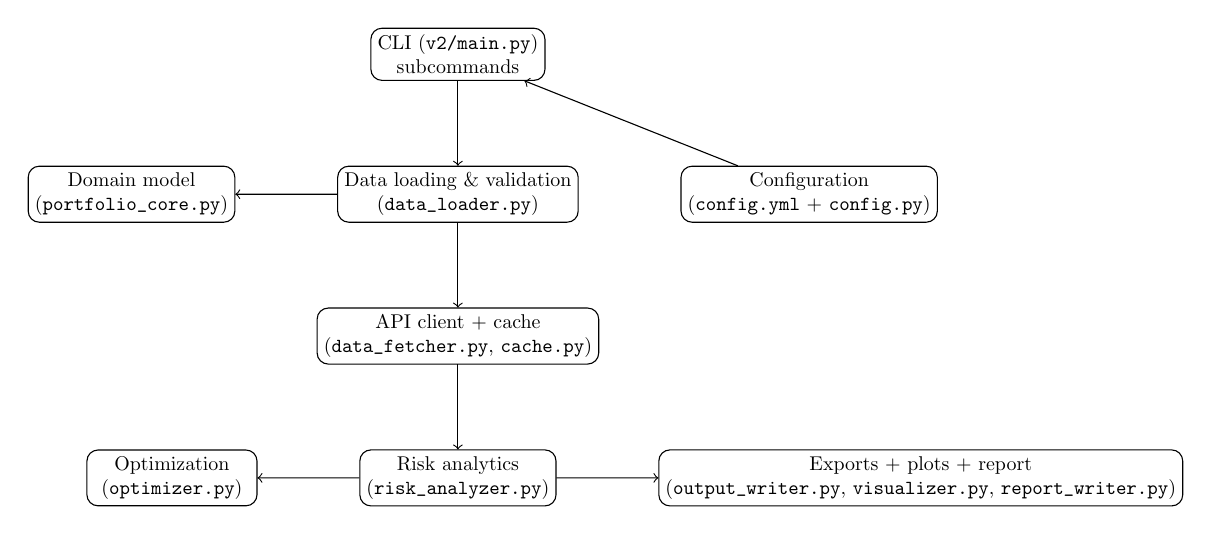
\begin{tikzpicture}[node distance=1.5cm, scale=0.72, transform shape]
  \tikzstyle{box}=[draw, rounded corners, minimum width=3.0cm, minimum height=0.9cm, align=center]
  \node[box] (cli) {CLI (\verb|v2/main.py|)\\subcommands};
  \node[box, below=of cli] (loader) {Data loading \& validation\\(\verb|data_loader.py|)};
  \node[box, left=1.8cm of loader] (core) {Domain model\\(\verb|portfolio_core.py|)};
  \node[box, right=1.8cm of loader] (config) {Configuration\\(\verb|config.yml| + \verb|config.py|)};
  \node[box, below=of loader] (fetch) {API client + cache\\(\verb|data_fetcher.py|, \verb|cache.py|)};
  \node[box, below=of fetch] (risk) {Risk analytics\\(\verb|risk_analyzer.py|)};
  \node[box, left=1.8cm of risk] (opt) {Optimization\\(\verb|optimizer.py|)};
  \node[box, right=1.8cm of risk] (viz) {Exports + plots + report\\(\verb|output_writer.py|, \verb|visualizer.py|, \verb|report_writer.py|)};

  \draw[->] (cli) -- (loader);
  \draw[->] (loader) -- (fetch);
  \draw[->] (loader) -- (core);
  \draw[->] (config) -- (cli);
  \draw[->] (fetch) -- (risk);
  \draw[->] (risk) -- (opt);
  \draw[->] (risk) -- (viz);
\end{tikzpicture}
\caption{High-level architecture of v2.}
\label{fig:architecture}
\end{figure}

\subsection{Key data structures}

\begin{itemize}
    \item \textbf{Asset (dataclass, frozen):} Represents a single position with \texttt{symbol}, \texttt{amount}, and optionally \texttt{price} and \texttt{crypto\_id}. We made it immutable to avoid accidental changes.
    \item \textbf{Portfolio (class):} A collection of \texttt{Asset} instances with methods \texttt{total\_value()} and \texttt{weights()}.
    \item \textbf{Configuration dataclasses (e.g., \texttt{AppConfig}, \texttt{RiskConfig}):} typed parameters loaded from YAML so we don't hardcode values.
    \item \textbf{Cache entries (JSON):} Historical price series stored locally with timestamps, so we can work offline and reproduce results.
\end{itemize}

\subsection{Data pipeline}

The pipeline proceeds as follows:
\begin{enumerate}
    \item \textbf{Load and validate:} Parse the portfolio JSON, check required fields, and instantiate \texttt{Asset} objects.
    \item \textbf{Fetch current prices:} Query the API for each asset's latest price.
    \item \textbf{Fetch historical prices:} Query daily prices over the configured window; cache results locally.
    \item \textbf{Align and transform:} Align all time series on common dates; compute simple returns.
    \item \textbf{Compute metrics:} Per-asset volatility, Sharpe, VaR; portfolio-level volatility and correlation matrix.
    \item \textbf{Export and visualize:} Write CSV/JSON, generate plots, and optionally render an HTML report.
\end{enumerate}

\subsection{Understanding the risk metrics}

Before we get into formulas, here's what each metric actually means:

\begin{description}
    \item[Volatility] measures how much an asset's price bounces around. Higher volatility means more uncertainty---both upside potential and downside risk.
    \item[Sharpe ratio] compares return to risk. A higher Sharpe means better ``risk-adjusted'' performance: you're getting more return per unit of volatility.
    \item[Value at Risk (VaR)] answers: ``What's the worst loss I might expect, 95\% of the time?'' It quantifies downside exposure.
    \item[Correlation] shows how assets move together. High correlation means they rise and fall in sync, which reduces diversification benefits.
    \item[Efficient frontier] shows the best possible risk/return trade-offs. Points on the frontier are ``optimal''---no other portfolio gives you higher return for the same risk.
\end{description}

\subsection{Risk metrics and formulas}

\paragraph{Returns.}
Simple returns are computed as:
\[
r_t = \frac{p_t}{p_{t-1}} - 1.
\]

\paragraph{Volatility.}
If $\sigma(r)$ is the standard deviation of returns, annualized volatility is:
\[
\sigma_{\mathrm{ann}} = \sigma(r)\sqrt{365}.
\]

\paragraph{Sharpe ratio.}
With annual risk-free rate $r_f$, the Sharpe ratio is:
\[
\mathrm{Sharpe} = \frac{\mathbb{E}[r - r_f/365]}{\sigma(r - r_f/365)}\sqrt{365}.
\]

\paragraph{Historical VaR.}
For confidence level $\alpha$ (e.g., 0.95), historical VaR is:
\[
\mathrm{VaR}_\alpha = Q_{1-\alpha}(r),
\]
where $Q$ denotes the empirical quantile. This is a non-parametric approach---we just use the actual distribution of past returns.

\paragraph{Correlation and portfolio volatility.}
The correlation matrix tells us about diversification: low average correlation means losses in one asset might be offset by gains in another. Portfolio volatility takes these correlations into account:
\[
\sigma_{\mathrm{portfolio}} = \sqrt{w^\top \Sigma w},
\]
where $w$ is the weight vector and $\Sigma$ is the covariance matrix.

\subsection{Optimization (Markowitz)}

In v2, optimization is performed under constraints:
\[
\sum_{i=1}^{n} w_i = 1, \quad w_i \in [0, w_{\max}],
\]
with three modes:
\begin{itemize}
    \item \textbf{min-vol:} minimize variance $w^\top \Sigma w$,
    \item \textbf{max-sharpe:} maximize $(\mu^\top w - r_f) / \sqrt{w^\top \Sigma w}$,
    \item \textbf{target-return:} minimize variance such that $\mu^\top w = r^\star$.
\end{itemize}

We approximate the efficient frontier by solving multiple target-return problems between the feasible minimum and maximum expected returns. If a target isn't feasible, we just skip it.

\subsection{Complexity considerations}

If $n$ is the number of assets and $T$ the number of aligned days:
\begin{itemize}
    \item Return computation: $O(nT)$,
    \item Covariance/correlation: $O(n^2 T)$,
    \item Optimization: iterative (SLSQP), practically fast for small $n$.
\end{itemize}

\medskip
\textbf{Code references (no code listing).} For detailed implementation and docstrings, see:
\begin{itemize}
    \item \verb|v2/risk_analyzer.py| (e.g., \verb|portfolio_volatility()|, \verb|correlation_matrix()|): risk metrics and portfolio aggregation,
    \item \verb|v2/optimizer.py| (e.g., \verb|max_sharpe()|, \verb|efficient_frontier()|): constraints, objectives, and efficient frontier,
    \item \verb|v2/data_fetcher.py| and \verb|v2/cache.py|: API client, caching, offline mode,
    \item \verb|v2/main.py|: CLI subcommands and I/O orchestration.
\end{itemize}

The v2 codebase is over 2,000 lines of Python across 12 modules, which meets the non-trivial implementation requirement.

%==============================================================================
\section{User Guide}
%==============================================================================

This section provides practical instructions for installing and running the application.

\subsection{Installation}

From the repository root:
\begin{verbatim}
python -m venv .venv
source .venv/bin/activate  # macOS / Linux
.venv\Scripts\activate     # Windows
pip install -r requirements.txt
\end{verbatim}

v0 uses the standard library only; dependencies in \verb|requirements.txt| are for v1/v2 (pandas, numpy, scipy, matplotlib, requests, pyyaml, pytest).

\subsection{Execution (commands)}

\textbf{v0 (static prices, deterministic):}
\begin{verbatim}
python v0/main.py --portfolio data/sample_portfolio.json
\end{verbatim}

\textbf{v1 (live prices, risk metrics):}
\begin{verbatim}
python v1/main.py --portfolio data/sample_portfolio.json --days 30
\end{verbatim}

\textbf{v2 (full CLI with subcommands):}
\begin{verbatim}
python v2/main.py analyze --portfolio data/sample_portfolio.json \
  --outdir outputs --pretty
python v2/main.py optimize --portfolio data/sample_portfolio.json \
  --mode max-sharpe --outdir outputs --pretty
python v2/main.py visualize --portfolio data/sample_portfolio.json \
  --outdir report/assets --report
\end{verbatim}

\subsection{Running tests}

From the repository root:
\begin{verbatim}
pytest v1/tests/ -v
pytest v2/tests/ -v
\end{verbatim}

\subsection{CLI options (v2 highlights)}

\begin{itemize}
    \item \verb|--pretty| prints human-readable tables in the console (exports unchanged).
    \item \verb|--offline| uses cache only (no network calls)---useful for reproducibility.
    \item \verb|--refresh-cache| bypasses cache and refreshes data from the API.
    \item \verb|--log-level| / \verb|--quiet| / \verb|--verbose| control console verbosity.
\end{itemize}

\subsection{Configuration examples}

v2 reads \verb|v2/config.yml| by default and supports CLI overrides for key parameters (days, risk-free rate, confidence, output directory). This way, you can set defaults once and override them as needed.

\medskip
\textbf{API key.} CryptoCompare works without an API key, but you're limited to ~100 calls/hour. For higher limits, set the environment variable \verb|CRYPTOCOMPARE_API_KEY|.

\subsection{Example inputs/outputs}

Example portfolio format (v1/v2):
\begin{verbatim}
{
  "name": "defi_portfolio",
  "assets": [
    {"symbol": "ETH", "crypto_id": "ETH", "amount": 1.5},
    {"symbol": "BTC", "crypto_id": "BTC", "amount": 0.1}
  ]
}
\end{verbatim}

%==============================================================================
\section{Example Outputs and Visualizations}
%==============================================================================

This section shows examples of the figures generated by v2 (Figure~\ref{fig:risk_and_corr} and Figure~\ref{fig:alloc_and_frontier}).

\begin{figure}[h]
\centering
\includegraphics[width=0.48\textwidth]{assets/risk_bars.png}\hfill
\includegraphics[width=0.48\textwidth]{assets/correlation_heatmap.png}
\caption{(Left) Per-asset annualized volatility (risk bars). (Right) Correlation heatmap between assets; values close to 1 indicate assets that move together.}
\label{fig:risk_and_corr}
\end{figure}

\begin{figure}[h]
\centering
\includegraphics[width=0.40\textwidth]{assets/allocation.png}\hfill
\includegraphics[width=0.58\textwidth]{assets/frontier.png}
\caption{(Left) Current portfolio allocation (weights by market value). (Right) Efficient frontier under the configured constraints (risk/return trade-offs).}
\label{fig:alloc_and_frontier}
\end{figure}

%==============================================================================
\section{Evaluation \& Discussion}
%==============================================================================

Now that we've covered the design and implementation, let's reflect on what we achieved, what was difficult, and what the limitations are.

\subsection{Level of completion per stage}

\begin{itemize}
    \item \textbf{v0:} Complete baseline with deterministic output. We validated the data model without any external dependencies.
    \item \textbf{v1:} Complete analytics pipeline with live prices, aligned returns, and standard metrics. All core risk features work.
    \item \textbf{v2:} Complete final stage with configuration, caching/offline mode, optimization, exports, plots, HTML report, and 9 test files.
\end{itemize}

\subsection{Testing strategy}

The test suite focuses on correctness and robustness:
\begin{itemize}
    \item Unit tests for portfolio computations and risk metrics (edge cases, zero values).
    \item Unit tests for cache round-trip and TTL behavior.
    \item Optimizer tests to make sure weights are valid and constraints are satisfied.
    \item CLI tests using mocking to avoid non-deterministic API calls.
\end{itemize}

We focused on deterministic and critical paths (parsing, metrics, cache integrity), and we check that plotting routines generate files without errors.

\subsection{Main difficulties encountered and mitigations}

We ran into several challenges during development:

\begin{itemize}
    \item \textbf{API rate limits and variability:} We added caching with TTL, a refresh option, and offline mode; tests mock API calls.
    \item \textbf{Time-series alignment:} We align on common dates and fail fast if the aligned series is too short.
    \item \textbf{Cross-platform execution:} We resolve paths so root-level commands work consistently.
    \item \textbf{Optimization feasibility:} We restrict targets to feasible ranges and skip infeasible points on the frontier.
    \item \textbf{Interpretability:} We provide an HTML report with a glossary and data-driven interpretation for non-finance users.
\end{itemize}

\subsection{Reproducibility and offline mode}

Reproducibility is critical for any data-driven analysis. The application supports:
\begin{itemize}
    \item \textbf{Local caching + offline mode:} historical series are cached with timestamps and can be re-used without network calls.
    \item \textbf{Structured exports:} CSV/JSON outputs can be archived and compared across runs.
\end{itemize}

\subsection{Known limitations}

There are several limitations we're aware of:
\begin{itemize}
    \item \textbf{Short samples:} With only 30 days of data, estimates of expected returns and covariance can be unstable. Increasing the window helps, but assumes stationarity.
    \item \textbf{Historical VaR is backward-looking:} It uses past returns and doesn't extrapolate tail risk beyond the sample. Extreme events not in the sample won't be captured.
    \item \textbf{Optimization sensitivity:} Markowitz optimization is sensitive to estimation noise and ignores transaction costs; results are indicative, not something you should follow blindly.
\end{itemize}

%==============================================================================
\section{Possible Extensions or Improvements}
%==============================================================================

The current implementation meets the project requirements, but several extensions could make it more useful:
\begin{itemize}
    \item \textbf{Alternative risk models:} parametric VaR or CVaR (expected shortfall) for tail risk.
    \item \textbf{Benchmark comparison:} compare against BTC-only or equal-weight baselines.
    \item \textbf{Realistic constraints:} turnover limits and transaction costs in optimization.
\end{itemize}

We left these as future work to keep the current scope manageable and stable.

%==============================================================================
\section{Conclusion}
%==============================================================================

The DeFi Portfolio Analyzer shows a complete staged development workflow and a clean modular architecture applied to a data-driven problem. We started from a minimal prototype (v0), then incrementally added API integration (v1) and advanced features (v2) without breaking anything.

The final version is a configurable and testable CLI tool with reproducible outputs, visualizations, and an HTML report that non-finance users can understand. The codebase is over 2,000 lines of Python organized into 12 modules, with a pytest suite of 14 test files.

\medskip
\textbf{Key learnings (technical and methodological):}
\begin{itemize}
    \item \textbf{Modular architecture:} separation of concerns makes the code easier to maintain and test.
    \item \textbf{CLI + logging:} argparse subcommands and consistent logs make the tool easier to use and debug.
    \item \textbf{Configuration + reproducibility:} YAML + typed config, caching, and exports let you repeat runs reliably.
    \item \textbf{Testing:} unit and CLI tests with mocking give you fast, deterministic feedback.
\end{itemize}

\medskip
We believe this project meets the requirements for a non-trivial Python application: it tackles a clearly defined problem with a well-structured codebase, follows best practices from the course (OOP, logging, argparse, configuration, testing, visualization), and produces meaningful, reproducible outputs.

\end{document}
